%==============================================================================
% EN4021 -- Advanced Digital Systems
% Multi-Master Shared System Bus with Split Transactions and UART Remote Access
%==============================================================================
\documentclass[11pt,a4paper]{article}

\usepackage[utf8]{inputenc}
\usepackage[T1]{fontenc}
\usepackage{lmodern}
\usepackage[margin=1in]{geometry}
\usepackage{amsmath,amssymb}
\usepackage{booktabs}
\usepackage{tabularx}
\usepackage{array}
\usepackage{graphicx}
\graphicspath{{images/}}
\usepackage{listings}
\usepackage{xcolor}
\usepackage{tikz}
\usetikzlibrary{arrows.meta, positioning, shapes.geometric, calc, fit, backgrounds}
\usepackage{caption}
\usepackage{microtype}
\usepackage[hidelinks]{hyperref}

\hypersetup{
    pdfauthor={Jayakody J.A.K., Attanayake A.Y., Rajinthan R.},
    pdftitle={System Bus Design -- EN4021 Advanced Digital Systems}
}

\captionsetup{font=small, labelfont=bf}
\setlength{\parskip}{0.4em}
\setlength{\parindent}{0pt}
\renewcommand{\arraystretch}{1.15}

% ---- shared TikZ styles: clean, monochrome line art -------------------------
\definecolor{inkblue}{RGB}{30, 60, 110}
\definecolor{inkgray}{RGB}{110, 115, 125}
\definecolor{fillsoft}{RGB}{242, 244, 248}
\definecolor{codebg}{RGB}{248, 248, 248}

\tikzset{
    blk/.style   ={draw=inkblue, line width=0.7pt, fill=white,
                   minimum width=2.6cm, minimum height=0.95cm,
                   align=center, font=\small, rounded corners=1.5pt},
    wideblk/.style={blk, minimum width=12.6cm},
    mem/.style   ={blk, fill=fillsoft},
    ghost/.style ={draw=inkgray, dashed, line width=0.6pt, fill=white,
                   minimum width=2.6cm, minimum height=0.95cm,
                   align=center, font=\small, rounded corners=1.5pt},
    st/.style    ={draw=inkblue, line width=0.7pt, fill=white, circle,
                   minimum size=1.15cm, align=center, font=\scriptsize\bfseries},
    ar/.style    ={-{Latex[length=2.2mm]}, line width=0.6pt, draw=inkblue},
    arg/.style   ={-{Latex[length=2.2mm]}, line width=0.6pt, draw=inkgray},
    lbl/.style   ={font=\scriptsize, inner sep=1.5pt},
    lane/.style  ={draw=inkblue, line width=0.6pt, fill=white,
                   minimum height=0.62cm, align=center, font=\scriptsize},
    lanealt/.style={lane, fill=fillsoft}
}

% ---- Verilog listing style --------------------------------------------------
\lstdefinestyle{vlog}{
    language=Verilog,
    basicstyle=\ttfamily\scriptsize,
    keywordstyle=\bfseries,
    commentstyle=\itshape\color{inkgray},
    numbers=left,
    numberstyle=\tiny\color{inkgray},
    numbersep=7pt,
    backgroundcolor=\color{codebg},
    frame=single,
    rulecolor=\color{inkgray},
    tabsize=4,
    showstringspaces=false,
    captionpos=b,
    breaklines=true,
    columns=fullflexible
}
\lstset{style=vlog}

\newcommand{\sig}[1]{\texttt{#1}}

%==============================================================================
\begin{document}

%------------------------------------------------------------------ title page
\begin{titlepage}
\centering
\vspace*{1.2cm}

{\large Department of Electronic and Telecommunication Engineering\par}
\vspace{0.35cm}
{\large University of Moratuwa, Sri Lanka\par}

\vspace{3.0cm}

{\Huge System Bus Design\par}
\vspace{0.8cm}
{\large Multi-Master Shared Bus with Split Transactions\\[0.2cm]
and UART Remote Bus Access\par}

\vspace{1.0cm}
{\large EN4021 -- Advanced Digital Systems\par}

\vspace{3.0cm}

\begin{tabular}{ll}
\textsc{Members:} & \textsc{Index No}\\[0.15cm]
Jayakody J.A.K.   & 220247J\\
Attanayake A.Y.   & 220051D\\
Rajinthan R.      & 220502M\\
\end{tabular}

\vfill
{Target board: Terasic DE2-115 (Intel Cyclone~IV~E, \texttt{EP4CE115F29C7})\par}
\vspace{0.2cm}
{September 2026\par}
\end{titlepage}

\newpage
\tableofcontents
\newpage

%==============================================================================
\section{Overview}

The System Bus is a synchronous, multi-master shared interconnect for FPGA
platforms. The implementation reported here targets the Intel Cyclone~IV~E
family on the Terasic DE2-115 board and provides a two-master, three-slave
memory-mapped bus with hardware split-transaction support and a UART link that
lets one board execute bus transactions on a second, identical board.

The bus carries a 14-bit address, an 8-bit write data path and an 8-bit read
data path, with an explicit request/grant arbitration scheme. Split transactions
let the slow slave release the bus while it fetches, so the rest of the system
continues to run instead of stalling behind it.

\subsection{Architecture}

The implemented design provides:

\begin{itemize}
    \item \textbf{Two masters.} Master~0 (\sig{master\_node\_uart}) is the
          high-priority master and additionally carries the UART link to the
          second board. Master~1 (\sig{master\_node}) is a plain local master
          at lower priority.
    \item \textbf{Three memory slaves.} Slave~0 is a 4~KB split-transaction
          RAM; Slaves~1 and~2 are single-cycle RAMs of 4~KB and 2~KB.
    \item \textbf{A central bus interconnect} (\sig{bus\_interconnect})
          containing the arbiter, the address decoder, the granted-master
          multiplexer and the slave response return multiplexer.
    \item \textbf{Split transaction support} for the long-latency slave, so a
          3-cycle read on Slave~0 does not block the other master.
    \item \textbf{UART remote bus access}, in which a command issued on
          Master~0 with \sig{cmd\_remote}~=~1 is executed on the other board's
          bus and its result returned.
    \item \textbf{A JTAG In-System Sources and Probes front-end}
          (\sig{bus\_issp\_driver}) that drives both master command ports and
          reports results and latencies without using any board pins.
\end{itemize}

\begin{figure}[htbp]
\centering
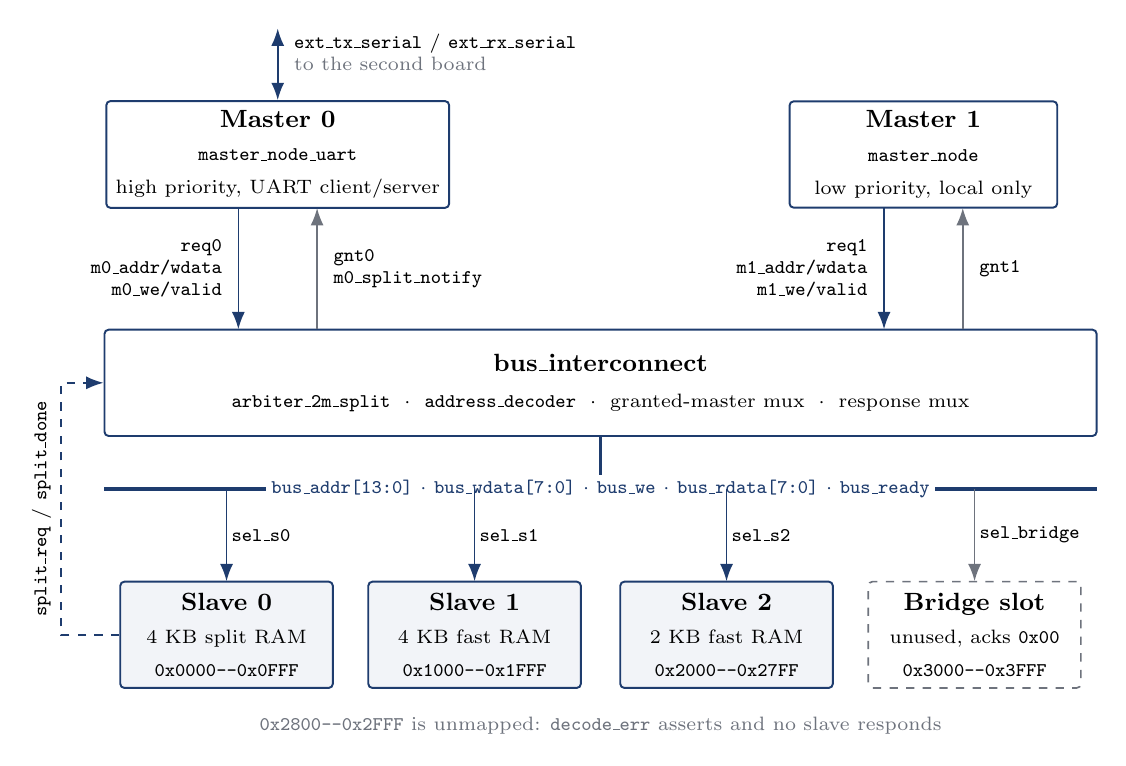
\begin{tikzpicture}[x=1cm, y=1cm]

  % ---- masters
  \node[blk, minimum width=3.4cm, minimum height=1.35cm] (m0) at (-4.1, 4.4)
       {\textbf{Master 0}\\[1pt]\scriptsize \sig{master\_node\_uart}\\[1pt]
        \scriptsize high priority, UART client/server};
  \node[blk, minimum width=3.4cm, minimum height=1.35cm] (m1) at ( 4.1, 4.4)
       {\textbf{Master 1}\\[1pt]\scriptsize \sig{master\_node}\\[1pt]
        \scriptsize low priority, local only};

  % ---- interconnect
  \node[blk, minimum width=12.6cm, minimum height=1.35cm] (ic) at (0, 1.5)
       {\textbf{bus\_interconnect}\\[2pt]
        \scriptsize \sig{arbiter\_2m\_split} $\;\cdot\;$ \sig{address\_decoder}
        $\;\cdot\;$ granted-master mux $\;\cdot\;$ response mux};

  % ---- master ports
  \draw[ar]  (-4.6, 3.72) -- (-4.6, 2.18);
  \draw[arg] (-3.6, 2.18) -- (-3.6, 3.72);
  \node[lbl, left, align=right] at (-4.75, 2.95)
       {\sig{req0}\\ \sig{m0\_addr/wdata}\\ \sig{m0\_we/valid}};
  \node[lbl, right, align=left] at (-3.45, 2.95)
       {\sig{gnt0}\\ \sig{m0\_split\_notify}};

  \draw[ar]  ( 3.6, 3.72) -- ( 3.6, 2.18);
  \draw[arg] ( 4.6, 2.18) -- ( 4.6, 3.72);
  \node[lbl, left, align=right] at (3.45, 2.95)
       {\sig{req1}\\ \sig{m1\_addr/wdata}\\ \sig{m1\_we/valid}};
  \node[lbl, right, align=left] at (4.75, 2.95)
       {\sig{gnt1}};

  % ---- shared bus rail
  \draw[line width=0.9pt, draw=inkblue] (0, 0.82) -- (0, 0.15);
  \draw[line width=1.2pt, draw=inkblue] (-6.3, 0.15) -- (6.3, 0.15);
  \node[lbl, fill=white, inner sep=2pt, text=inkblue] at (0, 0.15)
       {\sig{bus\_addr[13:0]} $\cdot$ \sig{bus\_wdata[7:0]} $\cdot$ \sig{bus\_we}
        $\cdot$ \sig{bus\_rdata[7:0]} $\cdot$ \sig{bus\_ready}};

  % ---- slaves
  \node[mem, minimum width=2.7cm, minimum height=1.35cm]   (s0) at (-4.75,-1.7)
       {\textbf{Slave 0}\\[1pt]\scriptsize 4~KB split RAM\\[1pt]
        \scriptsize \texttt{0x0000--0x0FFF}};
  \node[mem, minimum width=2.7cm, minimum height=1.35cm]   (s1) at (-1.6,-1.7)
       {\textbf{Slave 1}\\[1pt]\scriptsize 4~KB fast RAM\\[1pt]
        \scriptsize \texttt{0x1000--0x1FFF}};
  \node[mem, minimum width=2.7cm, minimum height=1.35cm]   (s2) at ( 1.6,-1.7)
       {\textbf{Slave 2}\\[1pt]\scriptsize 2~KB fast RAM\\[1pt]
        \scriptsize \texttt{0x2000--0x27FF}};
  \node[ghost, minimum width=2.7cm, minimum height=1.35cm] (sb) at ( 4.75,-1.7)
       {\textbf{Bridge slot}\\[1pt]\scriptsize unused, acks \texttt{0x00}\\[1pt]
        \scriptsize \texttt{0x3000--0x3FFF}};

  \draw[ar]  (-4.75, 0.15) -- (-4.75,-1.02) node[lbl, midway, right] {\sig{sel\_s0}};
  \draw[ar]  (-1.6,  0.15) -- (-1.6, -1.02) node[lbl, midway, right] {\sig{sel\_s1}};
  \draw[ar]  ( 1.6,  0.15) -- ( 1.6, -1.02) node[lbl, midway, right] {\sig{sel\_s2}};
  \draw[arg] ( 4.75, 0.15) -- ( 4.75,-1.02) node[lbl, midway, right] {\sig{sel\_bridge}};

  % ---- split handshake back to the arbiter
  \draw[ar, dashed] (s0.west) -- (-6.85,-1.7) -- (-6.85, 1.5) -- (ic.west);
  \node[lbl, align=center, rotate=90] at (-7.1, -0.1)
       {\sig{split\_req} / \sig{split\_done}};

  % ---- UART link
  \draw[{Latex[length=2.2mm]}-{Latex[length=2.2mm]}, line width=0.6pt, draw=inkblue]
       (m0.north) -- (-4.1, 6.0);
  \node[lbl, right, align=left] at (-3.95, 5.7)
       {\sig{ext\_tx\_serial} / \sig{ext\_rx\_serial}\\
        \textcolor{inkgray}{to the second board}};

  % ---- note
  \node[lbl, text=inkgray] at (0,-2.85)
       {\texttt{0x2800--0x2FFF} is unmapped: \sig{decode\_err} asserts and no slave responds};
\end{tikzpicture}
\caption{Full system architecture. One master owns the shared bus at a time;
the interconnect multiplexes the granted master onto the bus and returns the
selected slave's response.}
\label{fig:arch}
\end{figure}

\subsection{Key Features}

\begin{itemize}
    \item \textbf{Multi-master support.} Two masters with deterministic
          fixed-priority arbitration (Master~0 prioritised), with one override:
          a pending split whose data has arrived jumps the queue.
    \item \textbf{Split transactions.} Slave~0 cannot answer a read
          immediately. It pulses \sig{split\_req}, and the arbiter revokes the
          grant and hands the bus to Master~1 while Slave~0 fetches in the
          background. \sig{split\_done} brings the original master back.
    \item \textbf{UART remote bus access.} Master~0 is symmetric: it is the
          \emph{client} for our own remote commands and the \emph{server} for
          the other board's, and both run through one shared \sig{master\_node}
          core.
    \item \textbf{Fail-safe remote link.} A remote transaction that gets no
          answer within \sig{RESP\_TIMEOUT} completes with \sig{cmd\_error} set
          rather than hanging the bus.
    \item \textbf{Embedded memory.} All three slave memories are full-depth
          \sig{altsyncram} instances mapped into M9K blocks, so memory costs
          block RAM rather than logic.
    \item \textbf{Pin-free verification.} The whole bus is exercised over JTAG
          through In-System Sources and Probes; only twelve pins leave the
          device.
\end{itemize}

%==============================================================================
\section{Address Allocation}

\subsection{General Address Encoding}

A 14-bit address is used, giving a 16~KB address space. The slave is selected
from the upper address bits by \sig{address\_decoder}; the remaining low-order
bits index the word inside the selected memory. Slaves 0 and 1 consume
\sig{addr[11:0]} (4~K words each) and Slave~2 consumes \sig{addr[10:0]}
(2~K words).

\begin{table}[htbp]
\centering
\caption{Decode fields}
\label{tab:decode}
\small
\begin{tabular}{llll}
\toprule
\textbf{Match} & \textbf{Select} & \textbf{Target} & \textbf{Local address} \\
\midrule
\sig{addr[13:12] == 2'b00}  & \sig{sel\_s0}     & Slave 0, 4~KB split RAM & \sig{addr[11:0]} \\
\sig{addr[13:12] == 2'b01}  & \sig{sel\_s1}     & Slave 1, 4~KB fast RAM  & \sig{addr[11:0]} \\
\sig{addr[13:11] == 3'b100} & \sig{sel\_s2}     & Slave 2, 2~KB fast RAM  & \sig{addr[10:0]} \\
\sig{addr[13:12] == 2'b11}  & \sig{sel\_bridge} & Bridge slot (unused)    & --- \\
\midrule
anything else               & \sig{decode\_err} & no target               & --- \\
\bottomrule
\end{tabular}
\end{table}

\subsection{Memory Map}

\begin{table}[htbp]
\centering
\caption{System memory map}
\label{tab:memmap}
\small
\begin{tabularx}{\textwidth}{llllX}
\toprule
\textbf{Range} & \textbf{Size} & \textbf{Target} & \textbf{Latency} & \textbf{Notes} \\
\midrule
\texttt{0x0000--0x0FFF} & 4~KB & Slave 0 (\sig{slave\_0\_split\_4k}) & write 1 clk, read split & Reads split; 3-cycle background fetch on a dual-port M9K. \\
\texttt{0x1000--0x1FFF} & 4~KB & Slave 1 (\sig{slave\_fast\_ram}, \sig{AW}=12) & 1 clk & Single-port M9K, \sig{ready <= sel}. \\
\texttt{0x2000--0x27FF} & 2~KB & Slave 2 (\sig{slave\_fast\_ram}, \sig{AW}=11) & 1 clk & Same module, half the depth. \\
\texttt{0x2800--0x2FFF} & 2~KB & \emph{unmapped} & --- & \sig{decode\_err} asserts; no slave answers (see Section~\ref{sec:limits}). \\
\texttt{0x3000--0x3FFF} & 4~KB & Bridge slot & 1 clk & Decoder slot kept for the bridge; answered with \sig{0x00} so it can never hang the bus. \\
\bottomrule
\end{tabularx}
\end{table}

\subsection{Addressing the Remote Board}

Remote access is \emph{not} address-mapped. Rather than reserving a window and
translating it, the command port of Master~0 carries an extra
\sig{cmd\_remote} qualifier:

\begin{itemize}
    \item \sig{cmd\_remote}~=~0 --- the transaction runs on the local bus and
          the address means what Table~\ref{tab:memmap} says.
    \item \sig{cmd\_remote}~=~1 --- the identical 14-bit address is carried
          over the UART and executed against the \emph{other board's} memory
          map, which is the same map on the same design.
\end{itemize}

The full 16~KB space is therefore reachable on either board, and a local
address and its remote twin are written the same way. The historical
\sig{cross\_fpga\_bridge} slave that occupied \texttt{0x3000--0x3FFF} has been
removed; the decoder slot survives only so that an access there is
acknowledged instead of hanging.

%==============================================================================
\section{Master Node}

\subsection{Purpose and Role}

\sig{master\_node} is the interface between a local command source (the ISSP
driver, or the UART server logic) and the shared bus. It latches a command,
raises \sig{bus\_req}, waits for the grant, drives address, write data and
write enable onto its master port, and returns read data with a one-cycle
\sig{cmd\_done} pulse. It also implements the master side of the split
protocol.

\subsection{Block Diagram}

\begin{figure}[htbp]
\centering
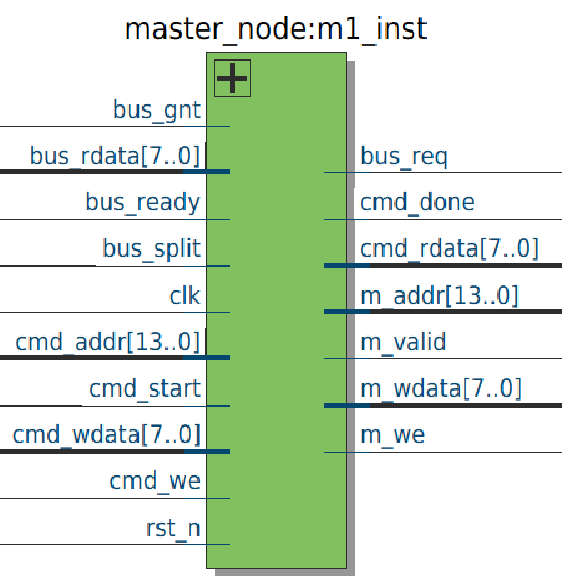
\includegraphics[width=0.52\textwidth]{Master.png}
\caption{\sig{master\_node} as elaborated by the Quartus RTL viewer
(instance \sig{m1\_inst}).}
\label{fig:blk_master}
\end{figure}

\subsection{I/O Description}

\begin{table}[htbp]
\centering
\caption{\sig{master\_node} I/O}
\label{tab:io_master}
\small
\begin{tabularx}{\textwidth}{llX}
\toprule
\textbf{Signal} & \textbf{Dir} & \textbf{Description} \\
\midrule
\sig{clk}, \sig{rst\_n} & Input  & 50~MHz clock; active-low asynchronous reset. \\
\sig{cmd\_start}        & Input  & One-cycle strobe that launches a transaction. \\
\sig{cmd\_we}           & Input  & 1 = write, 0 = read. \\
\sig{cmd\_addr[13:0]}   & Input  & Target bus address. \\
\sig{cmd\_wdata[7:0]}   & Input  & Write data. \\
\sig{cmd\_rdata[7:0]}   & Output & Read data, captured on reads only and held until the next read. \\
\sig{cmd\_done}         & Output & One-cycle completion pulse. \\
\sig{bus\_req}          & Output & Request to the arbiter; held through a split. \\
\sig{bus\_gnt}          & Input  & Grant from the arbiter. \\
\sig{bus\_split}        & Input  & Split notification from the arbiter. \\
\sig{m\_addr[13:0]}     & Output & Address driven to the master multiplexer. \\
\sig{m\_wdata[7:0]}     & Output & Write data driven to the master multiplexer. \\
\sig{m\_we}             & Output & Write enable driven to the master multiplexer. \\
\sig{m\_valid}          & Output & Qualifies the master port; gates the decoder. \\
\sig{bus\_rdata[7:0]}   & Input  & Read data return bus. \\
\sig{bus\_ready}        & Input  & Target acknowledge. \\
\bottomrule
\end{tabularx}
\end{table}

\subsection{State Diagram and Behaviour}

\begin{figure}[htbp]
\centering
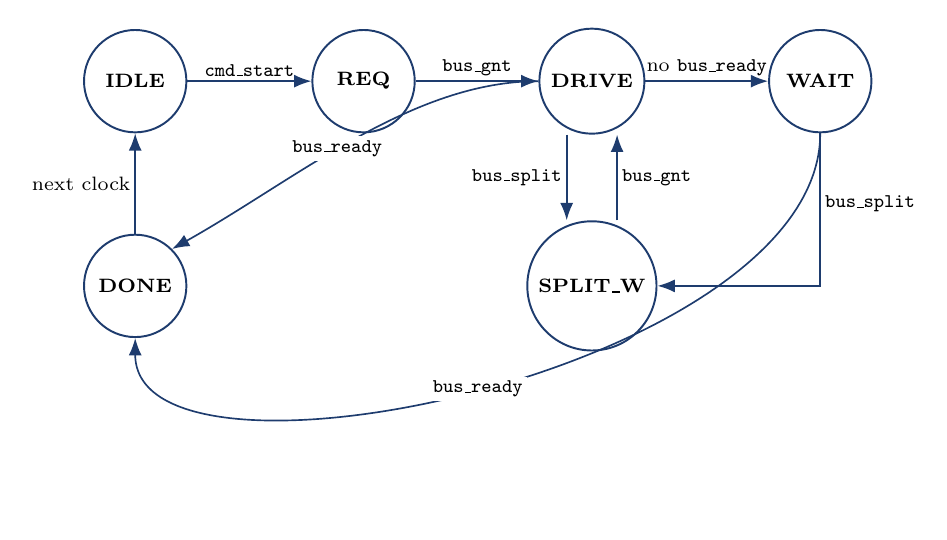
\begin{tikzpicture}[x=1cm, y=1cm]
  \node[st, minimum size=1.3cm] (idle)  at (0,0)    {IDLE};
  \node[st, minimum size=1.3cm] (req)   at (2.9,0)  {REQ};
  \node[st, minimum size=1.3cm] (drive) at (5.8,0)  {DRIVE};
  \node[st, minimum size=1.3cm] (wait)  at (8.7,0)  {WAIT};
  \node[st, minimum size=1.5cm] (split) at (5.8,-2.6) {SPLIT\_W};
  \node[st, minimum size=1.3cm] (done)  at (0,-2.6) {DONE};

  \draw[ar] (idle) -- node[lbl, above] {\sig{cmd\_start}} (req);
  \draw[ar] (req)  -- node[lbl, above] {\sig{bus\_gnt}} (drive);
  \draw[ar] (drive)-- node[lbl, above] {no \sig{bus\_ready}} (wait);

  % drive <-> split
  \draw[ar] ($(drive.south)+(-0.32,0)$) -- node[lbl, left] {\sig{bus\_split}}
            ($(split.north)+(-0.32,0)$);
  \draw[ar] ($(split.north)+(0.32,0)$) -- node[lbl, right] {\sig{bus\_gnt}}
            ($(drive.south)+(0.32,0)$);

  % wait -> split
  \draw[ar] (wait.south) -- (8.7,-2.6) node[lbl, above right, pos=0.55] {\sig{bus\_split}} -- (split.east);

  % completion
  \draw[ar] (drive.west) .. controls +(-1.6,0) and +(1.6,0.9) ..
            node[lbl, fill=white, pos=0.55] {\sig{bus\_ready}} (done.north east);
  \draw[ar] (wait.south) .. controls +(0,-3.0) and +(0,-2.2) ..
            node[lbl, fill=white, pos=0.5] {\sig{bus\_ready}} (done.south);

  \draw[ar] (done) -- node[lbl, left] {next clock} (idle);
\end{tikzpicture}
\caption{\sig{master\_node} state machine. After a split the master returns to
\sig{DRIVE} on the re-grant and completes there.}
\label{fig:fsm_master}
\end{figure}

\begin{itemize}
    \item \textbf{IDLE.} Waits for \sig{cmd\_start}. On the strobe it latches
          address, data and direction into internal registers, asserts
          \sig{bus\_req} and moves to \sig{REQ}.
    \item \textbf{REQ.} Waits for \sig{bus\_gnt}. On the grant it drives
          \sig{m\_addr}, \sig{m\_wdata}, \sig{m\_we} and raises \sig{m\_valid}.
    \item \textbf{DRIVE.} If \sig{bus\_split} is asserted it drops
          \sig{m\_valid}, \emph{keeps} \sig{bus\_req} high and parks in
          \sig{SPLIT\_W}. If \sig{bus\_ready} is asserted the transaction
          completes: on a read the return data is captured, \sig{cmd\_done}
          pulses, and the FSM goes to \sig{DONE}. Otherwise it waits.
    \item \textbf{WAIT.} Same two exits as \sig{DRIVE}, for slaves that need
          more than one cycle to answer.
    \item \textbf{SPLIT\_W.} Holds \sig{bus\_req} while the slave fetches in the
          background. When the arbiter re-grants, the FSM re-issues the read
          from its latched address (forced to a read, write data zeroed) and
          returns to \sig{DRIVE} to collect the prepared data.
    \item \textbf{DONE.} Clears the control flags and returns to \sig{IDLE}.
\end{itemize}

Read data is captured only when \sig{reg\_we} is 0. The slave memories echo
\sig{din} onto \sig{dout} during a write, so capturing unconditionally would
overwrite the last read value with the byte just written --- and, since
\sig{cmd\_rdata} drives the LEDs, would visibly corrupt the display after every
write.

%==============================================================================
\section{UART Master Node}

\subsection{Purpose}

\sig{master\_node\_uart} is Master~0. It wraps an ordinary \sig{master\_node}
core and adds a UART client and a UART server around it, so that one block both
issues remote transactions and executes the other board's. There is no separate
bridge master and bridge slave: the same core performs every local bus access,
whoever asked for it.

\begin{itemize}
    \item \textbf{Client path:} \sig{cmd\_remote} $\rightarrow$ send REQUEST
          $\rightarrow$ wait for RESPONSE $\rightarrow$ \sig{cmd\_rdata},
          \sig{cmd\_done}.
    \item \textbf{Server path:} REQUEST arrives $\rightarrow$ run it on the
          local bus through the core $\rightarrow$ send RESPONSE.
\end{itemize}

\subsection{Block Diagram}

\begin{figure}[htbp]
\centering
\includegraphics[width=0.46\textwidth]{{UART controlling master}}
\caption{\sig{master\_node\_uart} (instance \sig{m0\_inst}). Beyond the ordinary
master ports it carries \sig{cmd\_remote}, \sig{cmd\_error} and the two serial
pins.}
\label{fig:blk_uartmaster}
\end{figure}

\begin{figure}[htbp]
\centering
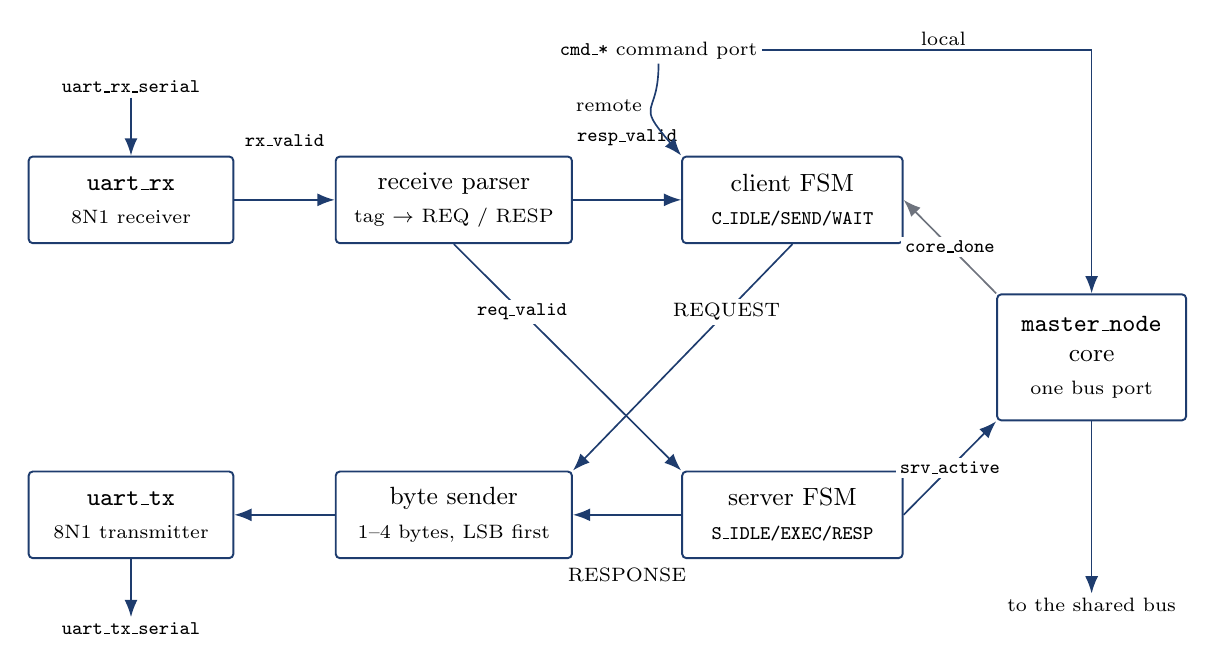
\begin{tikzpicture}[x=1cm, y=1cm]
  \node[blk, minimum width=2.6cm, minimum height=1.1cm] (rx)  at (-6.4, 2.0)
       {\sig{uart\_rx}\\[1pt]\scriptsize 8N1 receiver};
  \node[blk, minimum width=2.6cm, minimum height=1.1cm] (tx)  at (-6.4,-2.0)
       {\sig{uart\_tx}\\[1pt]\scriptsize 8N1 transmitter};
  \node[blk, minimum width=3.0cm, minimum height=1.1cm] (par) at (-2.3, 2.0)
       {receive parser\\[1pt]\scriptsize tag $\rightarrow$ REQ / RESP};
  \node[blk, minimum width=3.0cm, minimum height=1.1cm] (ser) at (-2.3,-2.0)
       {byte sender\\[1pt]\scriptsize 1--4 bytes, LSB first};
  \node[blk, minimum width=2.8cm, minimum height=1.1cm] (cli) at ( 2.0, 2.0)
       {client FSM\\[1pt]\scriptsize \sig{C\_IDLE/SEND/WAIT}};
  \node[blk, minimum width=2.8cm, minimum height=1.1cm] (srv) at ( 2.0,-2.0)
       {server FSM\\[1pt]\scriptsize \sig{S\_IDLE/EXEC/RESP}};
  \node[blk, minimum width=2.4cm, minimum height=1.6cm] (core) at ( 5.8, 0)
       {\sig{master\_node}\\ core\\[1pt]\scriptsize one bus port};

  % serial pins, entering from outside the block
  \draw[ar] (-6.4, 3.3) node[lbl, above] {\sig{uart\_rx\_serial}} -- (rx.north);
  \draw[ar] (tx.south) -- (-6.4,-3.3) node[lbl, below] {\sig{uart\_tx\_serial}};

  % receive and transmit chains
  \draw[ar] (rx)  -- node[lbl, above=0.62cm] {\sig{rx\_valid}} (par);
  \draw[ar] (par) -- node[lbl, above=0.62cm] {\sig{resp\_valid}} (cli);
  \draw[ar] (srv) -- node[lbl, below=0.62cm] {RESPONSE} (ser);
  \draw[ar] (ser) -- (tx);

  % crossing pair, labelled close to their sources
  \draw[ar] (par.south) -- node[lbl, fill=white, pos=0.3] {\sig{req\_valid}} (srv.north west);
  \draw[ar] (cli.south) -- node[lbl, fill=white, pos=0.3] {REQUEST} (ser.north east);

  % command port
  \node[lbl, align=center] (cmdp) at (0.3, 3.9) {\sig{cmd\_*} command port};
  \draw[ar] (cmdp.south) .. controls +(0,-0.7) and +(-0.6,0.7) .. (cli.north west);
  \node[lbl, left] at (0.15, 3.2) {remote};
  \draw[ar] (cmdp.east) -- (5.8, 3.9) node[lbl, above, pos=0.55] {local} -- (core.north);

  % core interface
  \draw[ar]  (srv.east) -- node[lbl, fill=white, pos=0.5] {\sig{srv\_active}} (core.south west);
  \draw[arg] (core.north west) -- node[lbl, fill=white, pos=0.5] {\sig{core\_done}} (cli.east);
  \draw[ar]  (core.south) -- (5.8,-3.0) node[lbl, below] {to the shared bus};
\end{tikzpicture}
\caption{Internal structure of \sig{master\_node\_uart}. \sig{srv\_active}
multiplexes the command inputs of the shared core between the local command
port and an incoming remote request.}
\label{fig:uart_internal}
\end{figure}

\subsection{I/O Description}

\begin{table}[htbp]
\centering
\caption{\sig{master\_node\_uart} I/O (additions to \sig{master\_node})}
\label{tab:io_uartmaster}
\small
\begin{tabularx}{\textwidth}{llX}
\toprule
\textbf{Signal} & \textbf{Dir} & \textbf{Description} \\
\midrule
\sig{cmd\_remote}     & Input  & 1 = execute this transaction on the other board. \\
\sig{cmd\_error}      & Output & Set with \sig{cmd\_done} when a remote transaction timed out. \\
\sig{uart\_rx\_serial}& Input  & Serial input from the other board. \\
\sig{uart\_tx\_serial}& Output & Serial output to the other board. \\
\sig{remote\_busy}    & Output & A remote transaction is outstanding. \\
\sig{srv\_busy}       & Output & Currently serving the other board's request. \\
\midrule
\multicolumn{3}{l}{\emph{Parameters}} \\
\sig{CLKS\_PER\_BIT}  & --- & Baud divisor, default 434 (50~MHz / 115200). \\
\sig{RESP\_TIMEOUT}   & --- & Response timeout in clocks, default 500\,000 ($\approx$10~ms). \\
\bottomrule
\end{tabularx}
\end{table}

All other ports are identical to \sig{master\_node} and pass straight through to
the core.

\subsection{Wire Format}

Frames are tagged so a request and a response can never be confused, which
matters because both directions share one physical link.

\begin{figure}[htbp]
\centering
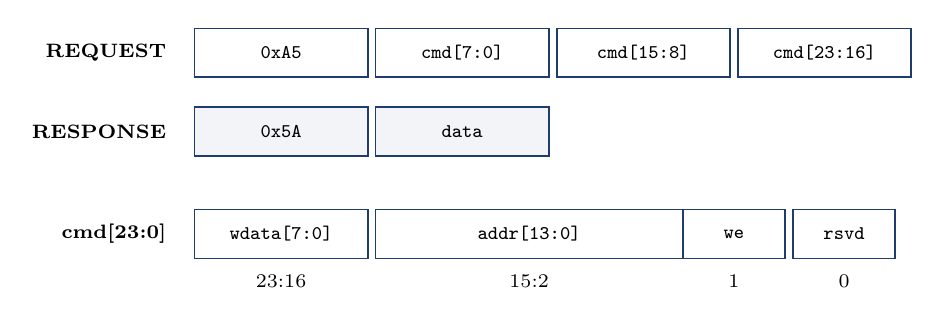
\begin{tikzpicture}
  % request
  \node[lbl, left] at (-0.2, 1.0) {\textbf{REQUEST}};
  \node[lane, minimum width=2.2cm] at (1.2, 1.0) {\texttt{0xA5}};
  \node[lane, minimum width=2.2cm] at (3.5, 1.0) {\texttt{cmd[7:0]}};
  \node[lane, minimum width=2.2cm] at (5.8, 1.0) {\texttt{cmd[15:8]}};
  \node[lane, minimum width=2.2cm] at (8.1, 1.0) {\texttt{cmd[23:16]}};
  % response
  \node[lbl, left] at (-0.2, 0.0) {\textbf{RESPONSE}};
  \node[lanealt, minimum width=2.2cm] at (1.2, 0.0) {\texttt{0x5A}};
  \node[lanealt, minimum width=2.2cm] at (3.5, 0.0) {\texttt{data}};

  % command layout
  \node[lbl, left] at (-0.2,-1.3) {\textbf{cmd[23:0]}};
  \node[lane, minimum width=2.2cm] at (1.2,-1.3)  {\texttt{wdata[7:0]}};
  \node[lane, minimum width=3.9cm] at (4.35,-1.3) {\texttt{addr[13:0]}};
  \node[lane, minimum width=1.3cm] at (6.95,-1.3) {\texttt{we}};
  \node[lane, minimum width=1.3cm] at (8.35,-1.3) {\texttt{rsvd}};
  \node[lbl] at (1.2,-1.9)  {23:16};
  \node[lbl] at (4.35,-1.9) {15:2};
  \node[lbl] at (6.95,-1.9) {1};
  \node[lbl] at (8.35,-1.9) {0};
\end{tikzpicture}
\caption{UART frame formats (8N1) and the 24-bit command layout, which uses the
same field order as one ISSP source slice.}
\label{fig:frames}
\end{figure}

Bytes go out least-significant first. A write brings back a response carrying
\sig{0x00} as an acknowledgement, so \sig{cmd\_done} on a remote write means the
far side really performed it.

\subsection{State Machine Logic}

\textbf{Client (\sig{cs}).}
\begin{itemize}
    \item \textbf{C\_IDLE:} on \sig{cmd\_start} with \sig{cmd\_remote}, packs
          \sig{\{cmd\_wdata, cmd\_addr, cmd\_we, 1'b0\}} into \sig{out\_cmd}.
    \item \textbf{C\_SEND:} once the shared transmitter is free, queues the
          four-byte request and clears the timeout counter.
    \item \textbf{C\_WAIT:} completes on \sig{resp\_valid} with the returned
          byte, or after \sig{RESP\_TIMEOUT} clocks with \sig{cmd\_rdata} =
          \sig{0xFF} and \sig{cmd\_error} set.
\end{itemize}

\textbf{Server (\sig{ss}).}
\begin{itemize}
    \item \textbf{S\_IDLE:} a latched incoming request is taken up when the core
          is not already running a local command; \sig{srv\_active} switches the
          core's command inputs to the remote fields.
    \item \textbf{S\_EXEC:} waits for \sig{core\_done}; a read captures
          \sig{core\_rdata}, a write yields \sig{0x00}.
    \item \textbf{S\_RESP:} queues the two-byte response and releases the core.
\end{itemize}

\textbf{Transmitter priority.} Responses take priority over requests in the
shared byte sender (\sig{C\_SEND} is held while \sig{ss == S\_RESP}). Without
that rule, two boards that issue remote commands on the same clock would both
sit in \sig{C\_WAIT} and neither would ever answer the other.

%==============================================================================
\section{Slave Ports}

\subsection{Slave 0 --- 4~KB Split RAM}

\subsubsection{Purpose}

\sig{slave\_0\_split\_4k} models a long-latency target. Writes complete in one
cycle, but a read takes \sig{SPLIT\_LATENCY}~=~3 background cycles, during which
the slave gives the bus up rather than stalling it.

The memory is one \sig{altsyncram} in simple dual-port mode: port~A is the
write path driven by the live bus address, and port~B is the read path driven
by the internally latched \sig{saved\_raddr}. Mapping the two logically
independent accesses onto the block's two real ports keeps the whole
4~K$\times$8 memory inside M9K blocks instead of spilling into logic.

\subsubsection{Block Diagram}

\begin{figure}[htbp]
\centering
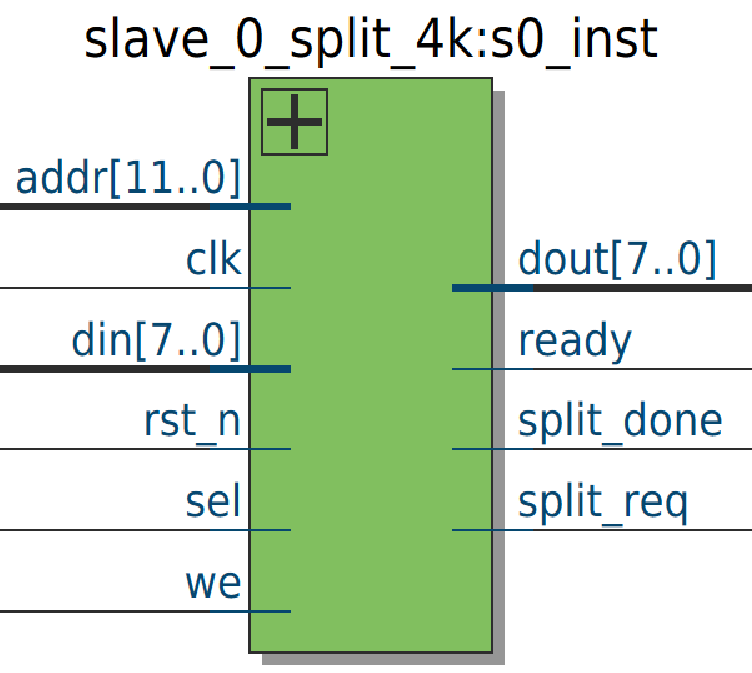
\includegraphics[width=0.44\textwidth]{Slave_4k.png}
\caption{\sig{slave\_0\_split\_4k} (instance \sig{s0\_inst}). The
\sig{split\_req}/\sig{split\_done} pair is what distinguishes it from the fast
slaves.}
\label{fig:blk_slave0}
\end{figure}

\subsubsection{I/O Description}

\begin{table}[htbp]
\centering
\caption{\sig{slave\_0\_split\_4k} I/O}
\label{tab:io_slave0}
\small
\begin{tabularx}{\textwidth}{llX}
\toprule
\textbf{Signal} & \textbf{Dir} & \textbf{Description} \\
\midrule
\sig{clk}, \sig{rst\_n} & Input  & Clock and active-low reset. \\
\sig{sel}               & Input  & Select from the decoder (\sig{sel\_s0}). \\
\sig{we}                & Input  & 1 = write, 0 = read. \\
\sig{addr[11:0]}        & Input  & Word address inside the 4~KB window. \\
\sig{din[7:0]}          & Input  & Write data. \\
\sig{dout[7:0]}         & Output & Read data, or the write echo. \\
\sig{ready}             & Output & Transaction acknowledge. \\
\sig{split\_req}        & Output & One-cycle strobe asking the arbiter to split. \\
\sig{split\_done}       & Output & One-cycle strobe when the background fetch has landed. \\
\bottomrule
\end{tabularx}
\end{table}

\subsubsection{Split Behaviour}

\begin{enumerate}
    \item A read arrives. The slave latches \sig{addr} into \sig{saved\_raddr},
          sets \sig{processing\_split}, pulses \sig{split\_req} and starts the
          latency counter.
    \item The counter runs in the background. Port~B of the M9K has had a stable
          address for the whole window, well beyond its one-cycle read latency,
          so at the terminal count \sig{ram\_q\_b} is captured into
          \sig{split\_data\_reg}, \sig{split\_done} pulses and
          \sig{data\_ready\_for\_fetch} is set.
    \item The master is re-granted and re-issues the same address. It matches
          \sig{saved\_raddr}, so the slave returns \sig{split\_data\_reg} with
          \sig{ready} and clears \sig{data\_ready\_for\_fetch}.
\end{enumerate}

The \sig{just\_completed} flag blocks the split-start branch for exactly one
cycle after a split is served. Without it, the master's \sig{m\_valid} (and
therefore \sig{sel}) is still high on the following cycle, the start condition
matches again, and the slave opens a phantom second split for the same
address --- which leaves a later read of any \emph{other} slave-0 address
matching neither branch, asserting neither \sig{ready} nor \sig{split\_req},
and deadlocking the bus.

\begin{figure}[htbp]
\centering
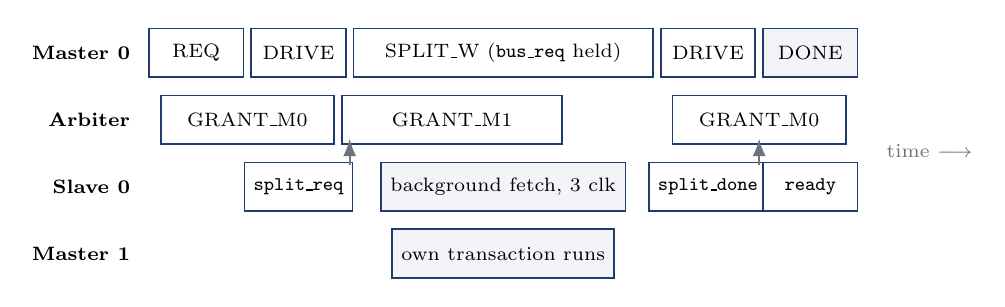
\begin{tikzpicture}[x=1.3cm, y=1.0cm]
  \node[lbl, left] at (-0.1, 0)    {\textbf{Master 0}};
  \node[lbl, left] at (-0.1,-0.85) {\textbf{Arbiter}};
  \node[lbl, left] at (-0.1,-1.7)  {\textbf{Slave 0}};
  \node[lbl, left] at (-0.1,-2.55) {\textbf{Master 1}};

  % master 0 lane
  \node[lane, minimum width=1.2cm] at (0.5, 0) {REQ};
  \node[lane, minimum width=1.2cm] at (1.5, 0) {DRIVE};
  \node[lane, minimum width=3.8cm] at (3.5, 0) {SPLIT\_W (\sig{bus\_req} held)};
  \node[lane, minimum width=1.2cm] at (5.5, 0) {DRIVE};
  \node[lanealt,minimum width=1.2cm] at (6.5, 0) {DONE};

  % arbiter lane
  \node[lane, minimum width=2.2cm] at (1.0,-0.85) {GRANT\_M0};
  \node[lane, minimum width=2.8cm] at (3.0,-0.85) {GRANT\_M1};
  \node[lane, minimum width=2.2cm] at (6.0,-0.85) {GRANT\_M0};

  % slave lane
  \node[lane, minimum width=1.2cm] at (1.5,-1.7) {\sig{split\_req}};
  \node[lanealt,minimum width=2.8cm] at (3.5,-1.7) {background fetch, 3 clk};
  \node[lane, minimum width=1.2cm] at (5.5,-1.7) {\sig{split\_done}};
  \node[lane, minimum width=1.2cm] at (6.5,-1.7) {\sig{ready}};

  % master 1 lane
  \node[lanealt,minimum width=2.8cm] at (3.5,-2.55) {own transaction runs};

  \draw[arg] (2.0,-1.42) -- (2.0,-1.09);
  \draw[arg] (6.0,-1.42) -- (6.0,-1.09);
  \node[lbl, text=inkgray, right] at (7.2, -1.25) {time $\longrightarrow$};
\end{tikzpicture}
\caption{Split read on Slave 0. Master 1 gets real work done inside the window
Master 0 spends waiting; the lane widths are indicative, not exact cycle counts.}
\label{fig:splitseq}
\end{figure}

\subsection{Slaves 1 and 2 --- Fast Single-Port RAM}

\subsubsection{Purpose}

\sig{slave\_fast\_ram} is the ordinary target: a single-port \sig{altsyncram}
in \sig{NEW\_DATA\_NO\_NBE\_READ} mode, which gives exactly ``\sig{dout} =
\sig{din} on a write, \sig{dout} = stored word on a read'' one cycle later, with
no register stage stacked on top of the block's own synchronous read latency.
\sig{ready} is a registered copy of \sig{sel}, so every access completes in one
cycle. Depth is set by the \sig{ADDR\_WIDTH} parameter --- 12 for the 4~KB
Slave~1, 11 for the 2~KB Slave~2.

\subsubsection{Block Diagram}

\begin{figure}[htbp]
\centering
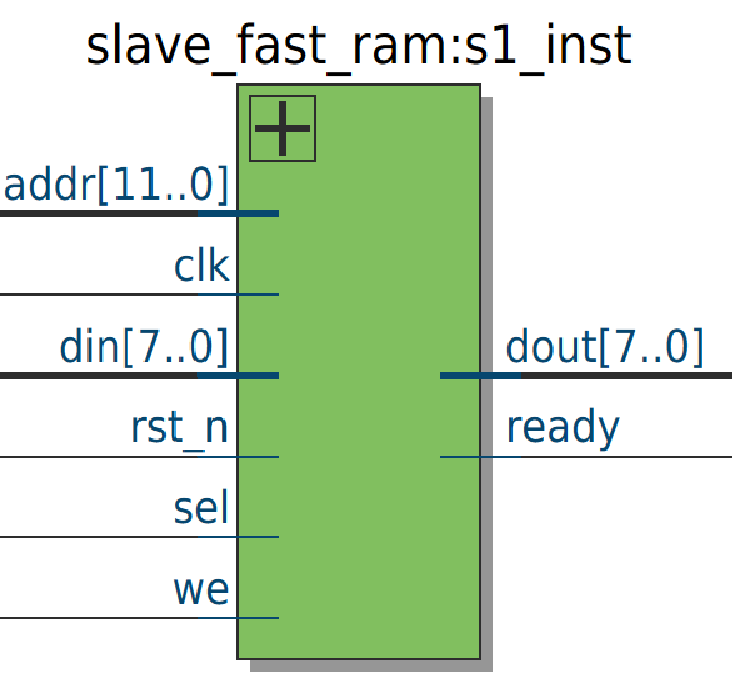
\includegraphics[width=0.44\textwidth]{Slave_2k.png}
\caption{\sig{slave\_fast\_ram} (instance \sig{s1\_inst}). Slave 2 is the same
module with \sig{ADDR\_WIDTH}~=~11.}
\label{fig:blk_slavefast}
\end{figure}

\subsubsection{I/O Description}

\begin{table}[htbp]
\centering
\caption{\sig{slave\_fast\_ram} I/O}
\label{tab:io_slavefast}
\small
\begin{tabularx}{\textwidth}{llX}
\toprule
\textbf{Signal} & \textbf{Dir} & \textbf{Description} \\
\midrule
\sig{clk}, \sig{rst\_n}      & Input  & Clock and active-low reset. \\
\sig{sel}                    & Input  & Select from the decoder (\sig{sel\_s1} or \sig{sel\_s2}). \\
\sig{we}                     & Input  & Write enable. \\
\sig{addr[AW-1:0]}           & Input  & Local word address. \\
\sig{din[7:0]}               & Input  & Write data. \\
\sig{dout[7:0]}              & Output & Read data, straight from the M9K output. \\
\sig{ready}                  & Output & One-cycle acknowledge, \sig{ready <= sel}. \\
\bottomrule
\end{tabularx}
\end{table}

%==============================================================================
\section{Arbiter}

\subsection{Overview}

\sig{arbiter\_2m\_split} serialises access to the shared bus. Priority is fixed:
Master~0 over Master~1. The one override is the split path --- a Master~0 split
whose data has arrived jumps ahead of a standing Master~1 request, because
otherwise the completed fetch could be starved indefinitely.

\subsection{I/O Description}

\begin{table}[htbp]
\centering
\caption{\sig{arbiter\_2m\_split} I/O}
\label{tab:io_arb}
\small
\begin{tabularx}{\textwidth}{llX}
\toprule
\textbf{Signal} & \textbf{Dir} & \textbf{Description} \\
\midrule
\sig{clk}, \sig{rst\_n}   & Input  & Clock and active-low reset. \\
\sig{req0}, \sig{req1}    & Input  & Requests from Master 0 (high priority) and Master 1. \\
\sig{gnt0}, \sig{gnt1}    & Output & Grants to Master 0 and Master 1. \\
\sig{s0\_split\_req}      & Input  & Split request from Slave 0. \\
\sig{s0\_split\_done}     & Input  & Background completion strobe from Slave 0. \\
\sig{m0\_split\_notify}   & Output & Tells Master 0 its transaction has been split. \\
\sig{m1\_split\_notify}   & Output & Declared for symmetry; never asserted (Section~\ref{sec:limits}). \\
\bottomrule
\end{tabularx}
\end{table}

Two internal status bits carry the split across states: \sig{m0\_split\_pending}
is set when a split starts under \sig{GRANT\_M0}, and \sig{split\_data\_ready}
latches the \sig{s0\_split\_done} pulse. Both clear when Master~0 re-acquires
the bus and completes.

\subsection{State Machine}

\begin{figure}[htbp]
\centering
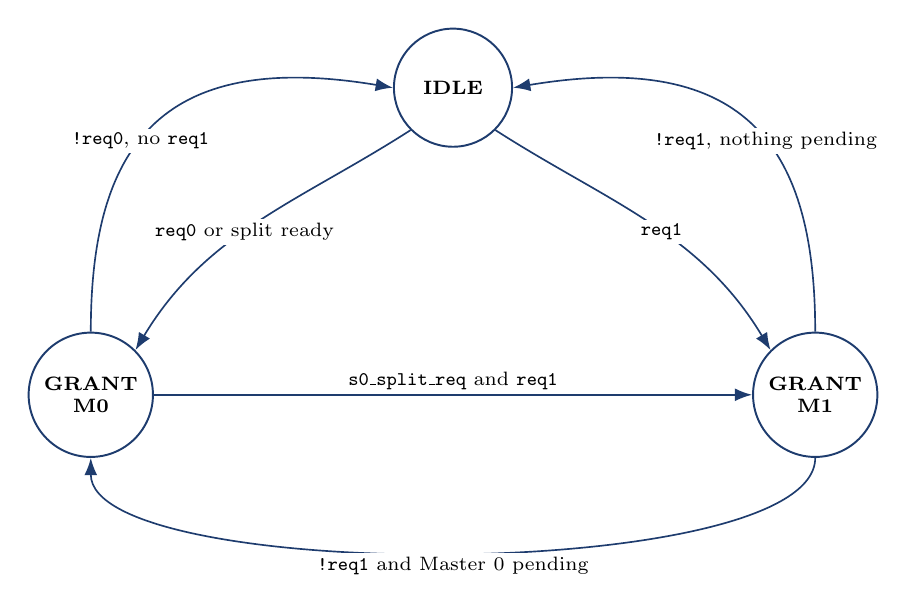
\begin{tikzpicture}[x=1cm, y=1cm]
  \node[st, minimum size=1.5cm] (idle) at (0, 2.6)     {IDLE};
  \node[st, minimum size=1.5cm] (g0)   at (-4.6,-1.3)  {GRANT\\M0};
  \node[st, minimum size=1.5cm] (g1)   at ( 4.6,-1.3)  {GRANT\\M1};

  \draw[ar] (idle.south west) .. controls +(-1.4,-0.9) and +(0.9,1.5) ..
        node[lbl, fill=white, pos=0.55] {\sig{req0} or split ready} (g0.north east);
  \draw[ar] (g0.north) .. controls +(0,2.3) and +(-3.0,0.5) ..
        node[lbl, fill=white, pos=0.45] {\sig{!req0}, no \sig{req1}} (idle.west);

  \draw[ar] (idle.south east) .. controls +(1.4,-0.9) and +(-0.9,1.5) ..
        node[lbl, fill=white, pos=0.55] {\sig{req1}} (g1.north west);
  \draw[ar] (g1.north) .. controls +(0,2.3) and +(3.0,0.5) ..
        node[lbl, fill=white, pos=0.45] {\sig{!req1}, nothing pending} (idle.east);

  \draw[ar] (g0.east) -- node[lbl, fill=white, above] {\sig{s0\_split\_req} and \sig{req1}} (g1.west);
  \draw[ar] (g1.south) .. controls +(0,-1.6) and +(0,-1.6) ..
        node[lbl, fill=white, below] {\sig{!req1} and Master 0 pending} (g0.south);
\end{tikzpicture}
\caption{\sig{arbiter\_2m\_split} state machine. From \sig{IDLE} the exits are
evaluated in priority order each cycle: a split whose data is ready, then
\sig{req0}, then \sig{req1}.}
\label{fig:fsm_arb}
\end{figure}

\begin{itemize}
    \item \textbf{IDLE.} Evaluated in strict order: a pending split whose data
          is ready wins; then a plain Master~0 request (suppressed while a split
          of its own is pending); then Master~1.
    \item \textbf{GRANT\_M0.} Drives \sig{gnt0}. If Slave~0 raises
          \sig{s0\_split\_req}, the arbiter asserts \sig{m0\_split\_notify} and
          immediately hands the bus to Master~1 if it wants it, otherwise
          returns to \sig{IDLE}. It also leaves when Master~0 drops its request.
    \item \textbf{GRANT\_M1.} Drives \sig{gnt1} and holds it until Master~1
          finishes; only then is a pending Master~0 split or request serviced.
          Master~1 is never pre-empted mid-transaction.
\end{itemize}

Because Master~0 is granted first, it often \emph{finishes} first even on the
slow split slave, with Master~1 absorbing the wait. That latency ordering is an
artefact of arbitration, not a property the protocol guarantees.

%==============================================================================
\section{Address Decoder}

\subsection{Purpose}

\sig{address\_decoder} is purely combinational. Whenever \sig{bus\_valid} is
high it decodes the upper address bits into one-hot slave selects; when
\sig{bus\_valid} is low every select is low, so a bus with no granted master
touches no slave.

\subsection{I/O Description}

\begin{table}[htbp]
\centering
\caption{\sig{address\_decoder} I/O}
\label{tab:io_dec}
\small
\begin{tabularx}{\textwidth}{llX}
\toprule
\textbf{Signal} & \textbf{Dir} & \textbf{Description} \\
\midrule
\sig{addr[13:0]}  & Input  & Address of the granted master. \\
\sig{bus\_valid}  & Input  & \sig{m\_valid} of the granted master; qualifies the decode. \\
\sig{sel\_s0}     & Output & Slave 0 select, \texttt{0x0000--0x0FFF}. \\
\sig{sel\_s1}     & Output & Slave 1 select, \texttt{0x1000--0x1FFF}. \\
\sig{sel\_s2}     & Output & Slave 2 select, \texttt{0x2000--0x27FF}. \\
\sig{sel\_bridge} & Output & Bridge slot select, \texttt{0x3000--0x3FFF}. \\
\sig{decode\_err} & Output & Unmapped access, \texttt{0x2800--0x2FFF}. \\
\bottomrule
\end{tabularx}
\end{table}

The decode is the priority chain of Table~\ref{tab:decode}: two-bit matches for
Slaves~0 and~1 and the bridge slot, a three-bit match for the half-size
Slave~2, and \sig{decode\_err} as the fall-through.

%==============================================================================
\section{Bus Interconnect}

\subsection{Module}

\sig{bus\_interconnect} is the fabric. It instantiates the arbiter and the
decoder and owns the three multiplexers that make a shared bus out of them:

\begin{enumerate}
    \item \textbf{Master multiplexer.} \sig{bus\_addr}, \sig{bus\_wdata},
          \sig{bus\_we} and \sig{bus\_valid} follow \sig{gnt0}, then
          \sig{gnt1}, and are driven to zero when neither is granted.
    \item \textbf{Decode.} The multiplexed address and valid drive
          \sig{address\_decoder}, producing the one-hot selects.
    \item \textbf{Response multiplexer.} \sig{bus\_rdata} and \sig{bus\_ready}
          are taken from whichever slave is selected, and are \sig{0x00} and
          \sig{0} when none is.
\end{enumerate}

Splitting this out of the top level keeps \sig{top\_bus\_system} to nothing but
instantiation and wiring, and means the arbitration and decode policy live in
one file.

\begin{figure}[htbp]
\centering
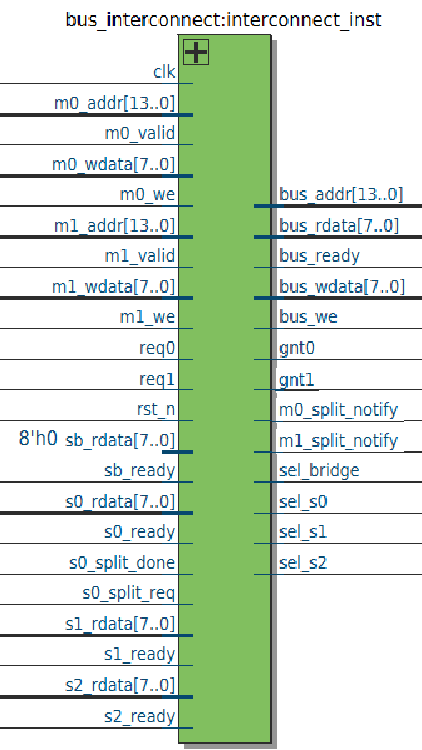
\includegraphics[width=0.38\textwidth]{Bus_Interconnect.png}
\caption{\sig{bus\_interconnect}. Both master port groups and every slave return
path enter on the left; the shared bus, the grants, the split notifications and
the one-hot selects leave on the right.}
\label{fig:blk_ic}
\end{figure}

\subsection{I/O Description}

\begin{table}[htbp]
\centering
\caption{\sig{bus\_interconnect} I/O}
\label{tab:io_ic}
\small
\begin{tabularx}{\textwidth}{llX}
\toprule
\textbf{Signal} & \textbf{Dir} & \textbf{Description} \\
\midrule
\sig{req0}, \sig{req1}                  & Input  & Requests from the two masters. \\
\sig{gnt0}, \sig{gnt1}                  & Output & Grants back to the masters. \\
\sig{m0\_split\_notify}, \sig{m1\_split\_notify} & Output & Split notifications from the arbiter. \\
\sig{m0\_addr}, \sig{m0\_wdata}, \sig{m0\_we}, \sig{m0\_valid} & Input & Master 0 port. \\
\sig{m1\_addr}, \sig{m1\_wdata}, \sig{m1\_we}, \sig{m1\_valid} & Input & Master 1 port. \\
\sig{bus\_addr}, \sig{bus\_wdata}, \sig{bus\_we} & Output & Shared bus driven to all slaves. \\
\sig{sel\_s0}, \sig{sel\_s1}, \sig{sel\_s2}, \sig{sel\_bridge} & Output & One-hot slave selects. \\
\sig{s0\_split\_req}, \sig{s0\_split\_done} & Input & Split handshake from Slave 0 to the arbiter. \\
\sig{s0/s1/s2/sb\_rdata}, \sig{\_ready} & Input  & Per-slave return data and acknowledge. \\
\sig{bus\_rdata}, \sig{bus\_ready}      & Output & Multiplexed response to the masters. \\
\bottomrule
\end{tabularx}
\end{table}

%==============================================================================
\section{UART Modules}

The physical link uses a plain 8N1 UART with a parameterised baud divisor,
\sig{CLKS\_PER\_BIT} = $f_\mathrm{clk}$/baud, which is 434 for 115\,200~baud at
50~MHz. Both halves are four-state machines (\sig{IDLE}, \sig{START},
\sig{DATA}, \sig{STOP}).

\sig{uart\_rx} double-flops \sig{rx\_serial} before use, since it arrives from a
pin and is asynchronous to \sig{clk}; it samples each bit at mid-bit and pulses
\sig{rx\_valid} for one cycle when a byte has been framed.

\begin{table}[htbp]
\centering
\caption{\sig{uart\_tx} and \sig{uart\_rx} I/O}
\label{tab:io_uart}
\small
\begin{tabularx}{\textwidth}{lllX}
\toprule
\textbf{Module} & \textbf{Signal} & \textbf{Dir} & \textbf{Description} \\
\midrule
\sig{uart\_tx} & \sig{tx\_start}   & Input  & One-cycle strobe; \sig{tx\_data} must be valid. \\
               & \sig{tx\_data}    & Input  & Byte to transmit. \\
               & \sig{tx\_serial}  & Output & Serial line, idles high. \\
               & \sig{tx\_busy}    & Output & High until the stop bit has been driven. \\
\midrule
\sig{uart\_rx} & \sig{rx\_serial}  & Input  & Serial line from the other board. \\
               & \sig{rx\_data}    & Output & Received byte. \\
               & \sig{rx\_valid}   & Output & One-cycle strobe when a byte is framed. \\
\bottomrule
\end{tabularx}
\end{table}

\subsection{Two-Board Topology}

\begin{figure}[htbp]
\centering
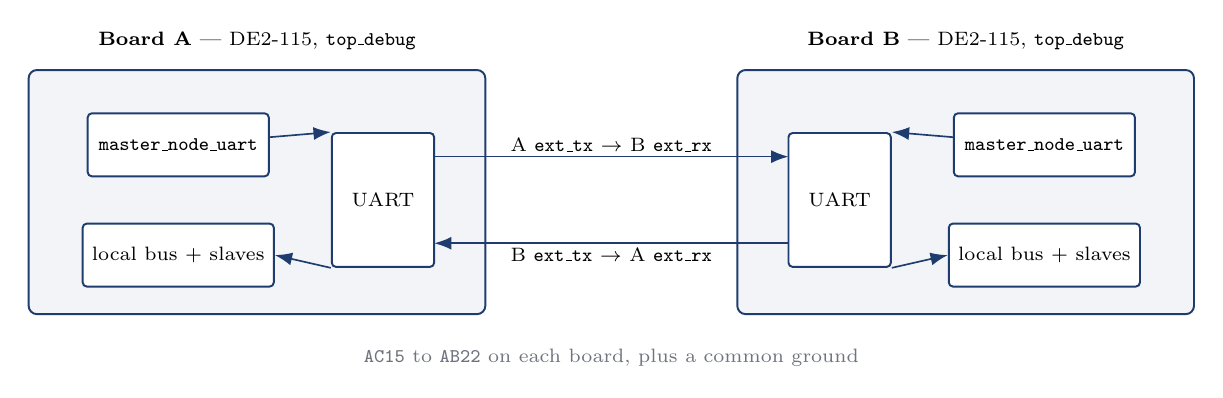
\begin{tikzpicture}[x=1cm, y=1cm]
  \node[draw=inkblue, line width=0.7pt, fill=fillsoft, rounded corners=3pt,
        minimum width=5.8cm, minimum height=3.1cm] (b1) at (-4.5,0) {};
  \node[lbl, above] at (-4.5,1.75) {\textbf{Board A} --- DE2-115, \sig{top\_debug}};
  \node[blk, minimum width=2.3cm, minimum height=0.8cm] (m0a) at (-5.5,0.6)
       {\scriptsize \sig{master\_node\_uart}};
  \node[blk, minimum width=2.3cm, minimum height=0.8cm] (sa)  at (-5.5,-0.8)
       {\scriptsize local bus + slaves};
  \node[blk, minimum width=1.3cm, minimum height=1.7cm] (ua)  at (-2.9,-0.1)
       {\scriptsize UART};

  \node[draw=inkblue, line width=0.7pt, fill=fillsoft, rounded corners=3pt,
        minimum width=5.8cm, minimum height=3.1cm] (b2) at ( 4.5,0) {};
  \node[lbl, above] at (4.5,1.75) {\textbf{Board B} --- DE2-115, \sig{top\_debug}};
  \node[blk, minimum width=2.3cm, minimum height=0.8cm] (m0b) at (5.5,0.6)
       {\scriptsize \sig{master\_node\_uart}};
  \node[blk, minimum width=2.3cm, minimum height=0.8cm] (sb)  at (5.5,-0.8)
       {\scriptsize local bus + slaves};
  \node[blk, minimum width=1.3cm, minimum height=1.7cm] (ub)  at (2.9,-0.1)
       {\scriptsize UART};

  \draw[ar] (m0a) -- (ua.north west);
  \draw[ar] (ua.south west) -- (sa.east);
  \draw[ar] (m0b) -- (ub.north east);
  \draw[ar] (ub.south east) -- (sb.west);

  \draw[ar] (-2.25,0.45) -- node[lbl, above] {A \sig{ext\_tx} $\rightarrow$ B \sig{ext\_rx}} (2.25,0.45);
  \draw[ar] ( 2.25,-0.65) -- node[lbl, below] {B \sig{ext\_tx} $\rightarrow$ A \sig{ext\_rx}} (-2.25,-0.65);
  \node[lbl, text=inkgray] at (0,-2.1) {\texttt{AC15} to \texttt{AB22} on each board, plus a common ground};
\end{tikzpicture}
\caption{Two identical boards with a crossed serial link. Either board can be
client or server, and both roles run concurrently.}
\label{fig:twoboard}
\end{figure}

%==============================================================================
\section{System Integration}

\sig{top\_bus\_system} instantiates the two masters, the interconnect and the
three slaves, and wires the bridge slot's acknowledge. \sig{top\_debug} is the
synthesis top: it adds \sig{bus\_issp\_driver} and exposes only \sig{clk},
\sig{rst\_n}, the two serial pins and \sig{led[7:0]}.

\begin{figure}[htbp]
\centering
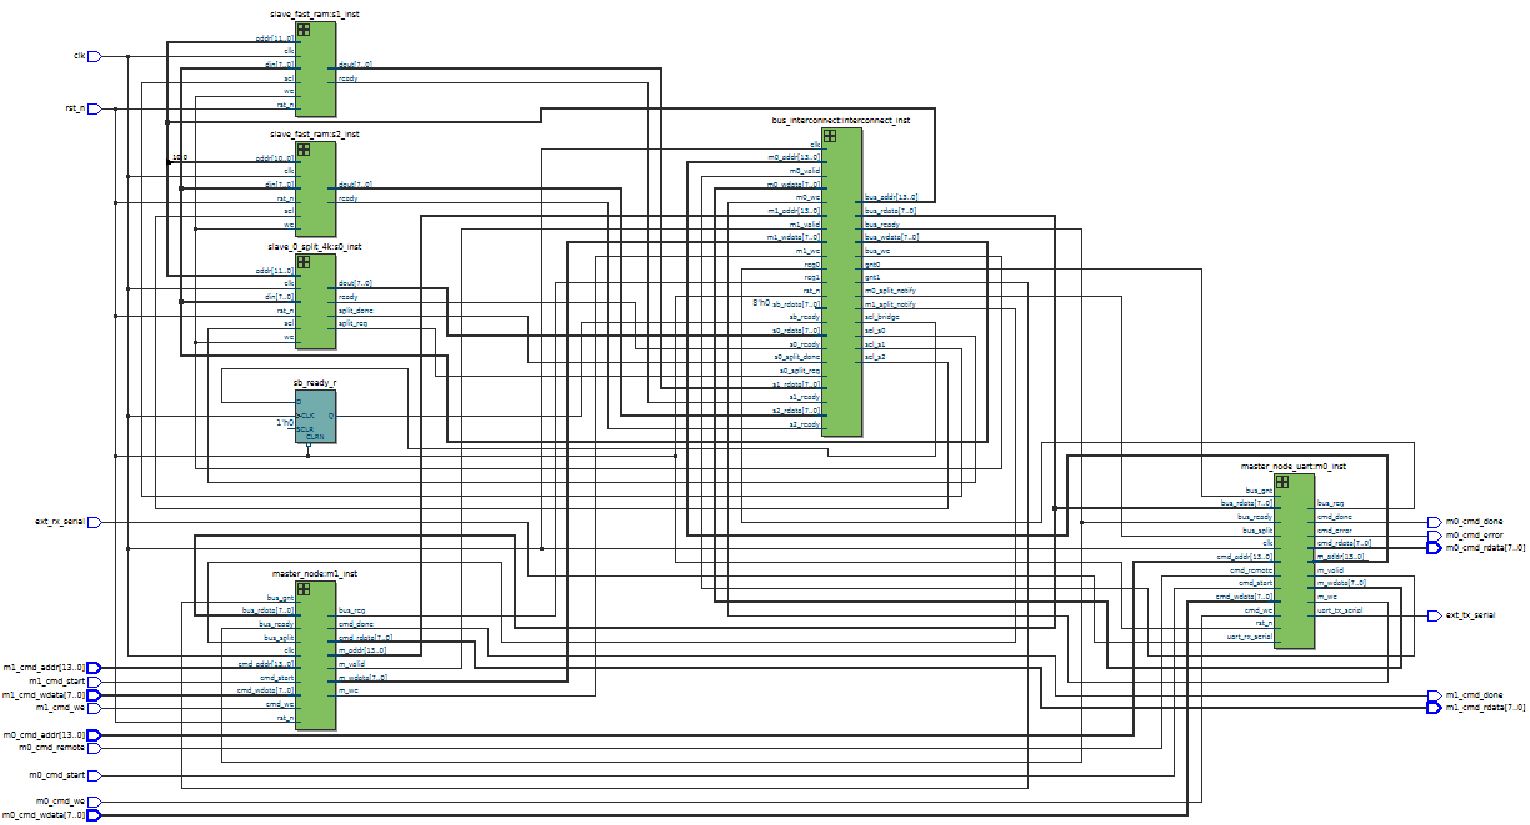
\includegraphics[width=\textwidth]{System.png}
\caption{Quartus RTL netlist of \sig{top\_bus\_system} as instantiated on the
device: both masters, the interconnect, the three slave memories and the
registered acknowledge for the unused bridge slot.}
\label{fig:rtl_system}
\end{figure}

The bridge slot deserves a note. The UART now lives inside Master~0, so nothing
is attached to \sig{sel\_bridge}. Leaving it dangling would make
\texttt{0x3000--0x3FFF} behave exactly like the unmapped gap, so the slot is
given a registered acknowledge returning \sig{0x00}:

\begin{lstlisting}[caption={Bridge slot acknowledge in \sig{top\_bus\_system}}]
reg sb_ready_r;
always @(posedge clk or negedge rst_n) begin
    if (!rst_n) sb_ready_r <= 1'b0;
    else        sb_ready_r <= sel_bridge;
end
assign sb_rdata = 8'h00;
assign sb_ready = sb_ready_r;
\end{lstlisting}

\sig{led[7:0]} shows \sig{m0\_cmd\_rdata}, which the master updates on reads
only, so the display holds the last byte read by Master~0.

%==============================================================================
\section{In-System Verification (JTAG ISSP)}

Routing 14 address lines and 8 data lines to switches was not practical, so both
master command ports are driven over JTAG through an Altera In-System Sources
and Probes instance (\sig{altsource\_probe}, instance ID \texttt{"BUS0"}), with
a 50-bit source and a 38-bit probe.

\subsection{Source Map (host $\rightarrow$ device, 50 bits)}

\begin{table}[htbp]
\centering
\caption{ISSP source bit map}
\label{tab:issp_src}
\small
\begin{tabularx}{\textwidth}{llX}
\toprule
\textbf{Bits} & \textbf{Field} & \textbf{Description} \\
\midrule
\sig{src[0]}     & \sig{m0\_go}         & Level; a 0$\rightarrow$1 edge launches one Master 0 command. \\
\sig{src[1]}     & \sig{m0\_cmd\_we}    & 1 = write, 0 = read. \\
\sig{src[15:2]}  & \sig{m0\_cmd\_addr}  & 14-bit bus address. \\
\sig{src[23:16]} & \sig{m0\_cmd\_wdata} & 8-bit write data. \\
\sig{src[24]}    & \sig{m1\_go}         & Master 1 launch level. \\
\sig{src[25]}    & \sig{m1\_cmd\_we}    & Master 1 direction. \\
\sig{src[39:26]} & \sig{m1\_cmd\_addr}  & Master 1 address. \\
\sig{src[47:40]} & \sig{m1\_cmd\_wdata} & Master 1 write data. \\
\sig{src[48]}    & \sig{soft\_rst}      & Clears the driver's sticky status flags. \\
\sig{src[49]}    & \sig{m0\_remote}     & 1 = execute this command on the other board. \\
\bottomrule
\end{tabularx}
\end{table}

\subsection{Probe Map (device $\rightarrow$ host, 38 bits)}

\begin{table}[htbp]
\centering
\caption{ISSP probe bit map}
\label{tab:issp_prb}
\small
\begin{tabularx}{\textwidth}{llX}
\toprule
\textbf{Bits} & \textbf{Field} & \textbf{Description} \\
\midrule
\sig{prb[7:0]}   & \sig{m0\_rl}     & Last read data captured for Master 0. \\
\sig{prb[8]}     & \sig{m0\_done\_s}& Sticky ``command finished''; clears when \sig{m0\_go} drops. \\
\sig{prb[9]}     & \sig{m0\_busy}   & Command in flight. \\
\sig{prb[17:10]} & \sig{m1\_rl}     & Last read data for Master 1. \\
\sig{prb[18]}    & \sig{m1\_done\_s}& Master 1 sticky done. \\
\sig{prb[19]}    & \sig{m1\_busy}   & Master 1 busy. \\
\sig{prb[27:20]} & \sig{m0\_lat}    & Clocks from launch to done, saturating at \sig{0xFF}. \\
\sig{prb[35:28]} & \sig{m1\_lat}    & Same for Master 1. \\
\sig{prb[36]}    & \sig{collision}  & Sticky: both masters were in flight at once. \\
\sig{prb[37]}    & \sig{m0\_error}  & Sticky: the last remote command timed out. \\
\bottomrule
\end{tabularx}
\end{table}

A latency reading of \sig{0xFF} with \sig{busy} still high means the transaction
never completed --- for instance an address in the \texttt{0x2800--0x2FFF}
decode gap, which asserts no select and therefore never returns
\sig{bus\_ready}.

\subsection{Test Procedure}

\sig{issp\_bus\_test.tcl} replays the \sig{tb\_top\_bus\_system.v} cases against
the real board and exits 0 on pass, 1 on failure. \sig{issp\_console.tcl} is the
interactive counterpart (\texttt{w} / \texttt{r} / \texttt{both} /
\texttt{sweep} against any slave and offset); \texttt{both} fires both masters
from a single source write so they reach the arbiter on the same clock.
Connection handling and the bit map are shared through \sig{issp\_bus\_lib.tcl}.

\begin{lstlisting}[language=bash, caption={Running the hardware tests},
                   basicstyle=\ttfamily\small, numbers=none]
cd System_Bus_Final
quartus_stp -t issp_bus_test.tcl        # the standard test run
quartus_stp -t issp_bus_test.tcl -gap   # + decode-gap deadlock demo
\end{lstlisting}

\sig{quartus\_stp} is the only interpreter that works. The Tcl packages
\sig{::quartus::jtag} and \sig{::quartus::insystem\_source\_probe} are
rejected outright by \sig{quartus\_sh}, and are absent from the GUI Tcl
console. To launch from the GUI,
\sig{run\_issp\_test.tcl} shells out to \sig{quartus\_stp} and echoes the output
back.

Two ordering constraints inside the script proved easy to trip over:

\begin{itemize}
    \item \sig{get\_insystem\_source\_probe\_instance\_info} opens a transient
          JTAG session of its own, so it must be called \emph{before}
          \sig{start\_insystem\_source\_probe}, never after.
    \item Bit 0 of each 24-bit source slice is the \sig{go} level and is
          deliberately excluded from the command payload
          (\sig{src[23:1]}, not \sig{src[23:0]}). Widening it back over bit 0
          aliases \sig{we} onto \sig{go} and makes reads impossible.
\end{itemize}

The In-System Sources and Probes editor tab must be closed before a scripted
run, since an open editor holds the JTAG session.

\subsection{Measured Latencies}

\begin{table}[htbp]
\centering
\caption{Transaction latency measured on hardware via \sig{m0\_lat}}
\label{tab:latency}
\small
\begin{tabular}{lll}
\toprule
\textbf{Transaction} & \textbf{Clocks} & \textbf{At 50~MHz} \\
\midrule
Fast slave read (Slave 1 or 2), uncontended & 6  & 120~ns \\
Split slave read (Slave 0), uncontended     & 12 & 240~ns \\
\bottomrule
\end{tabular}
\end{table}

%==============================================================================
\section{Timing Analysis}

The project as committed contains no \sig{.sdc} file, so the only clock the
Timing Analyzer sees is the JTAG \sig{altera\_reserved\_tck} and the system
clock is left unconstrained. For this report the fitted design was re-analysed
with the constraint below, applied to a scratch copy of the project.

\begin{lstlisting}[language=tcl, caption={Timing constraints used
(\sig{System\_Bus\_Final.sdc})}, numbers=none, basicstyle=\ttfamily\small]
create_clock -name clk -period 20.000 [get_ports {clk}]
derive_pll_clocks
derive_clock_uncertainty
set_false_path -from [get_ports {rst_n}]
set_false_path -from [get_ports {ext_rx_serial}]
set_false_path -to   [get_ports {ext_tx_serial}]
set_false_path -to   [get_ports {led[*]}]
\end{lstlisting}

\begin{table}[htbp]
\centering
\caption{Timing results for \sig{clk} constrained at 50~MHz
(Quartus Prime Lite 24.1std, \sig{EP4CE115F29C7})}
\label{tab:timing}
\small
\begin{tabular}{llll}
\toprule
\textbf{Check} & \textbf{Slow 1200\,mV 85\,\textdegree C} & \textbf{Slow 1200\,mV 0\,\textdegree C} & \textbf{Fast 1200\,mV 0\,\textdegree C} \\
\midrule
Setup slack             & 12.273~ns & 12.923~ns & 16.186~ns \\
Hold slack              &  0.402~ns &  0.353~ns &  0.181~ns \\
Minimum pulse width     &  9.554~ns &  9.560~ns &  9.201~ns \\
\bottomrule
\end{tabular}
\end{table}

Total negative slack is 0.000~ns on every check at every corner. The worst-case
corner reports \sig{Fmax} = \textbf{129.42~MHz} for \sig{clk}. Checked against
the 20~ns period directly,

\[
T_\mathrm{min} = 20\ \mathrm{ns} - 12.273\ \mathrm{ns} = 7.727\ \mathrm{ns},
\qquad
F_\mathrm{max} \approx \frac{1}{7.727\ \mathrm{ns}} \approx 129\ \mathrm{MHz},
\]

which agrees with the tool. The design meets 50~MHz with roughly $2.6\times$
margin, and hold is met at every corner. Adding this \sig{.sdc} to the project
is the single most worthwhile follow-up: without it, timing is never actually
signed off by the flow.

%==============================================================================
\section{Resource Utilisation}

\begin{table}[htbp]
\centering
\caption{Fitter resource usage, \sig{top\_debug} on \sig{EP4CE115F29C7}}
\label{tab:resources}
\small
\begin{tabular}{lll}
\toprule
\textbf{Resource} & \textbf{Used / available} & \textbf{Utilisation} \\
\midrule
Total logic elements            & 1{,}097 / 114{,}480 & $<1\%$ \\
\quad Combinational functions   &   734 / 114{,}480   & $<1\%$ \\
\quad Dedicated logic registers &   796 / 114{,}480   & $<1\%$ \\
Total registers                 &   796               & --- \\
Total pins                      &    12 / 529         & 2\% \\
Total memory bits               & 81{,}920 / 3{,}981{,}312 & 2\% \\
Embedded multipliers (9-bit)    &     0 / 532         & 0\% \\
Total PLLs                      &     0 / 4           & 0\% \\
\bottomrule
\end{tabular}
\end{table}

\begin{table}[htbp]
\centering
\caption{M9K block usage by slave}
\label{tab:m9k}
\small
\begin{tabular}{lllll}
\toprule
\textbf{Instance} & \textbf{Mode} & \textbf{Depth $\times$ width} & \textbf{Bits} & \textbf{M9Ks} \\
\midrule
\sig{s0\_inst} (\sig{slave\_0\_split\_4k}) & Simple dual port & $4096\times8$ & 32{,}768 & 4 \\
\sig{s1\_inst} (\sig{slave\_fast\_ram})    & Single port      & $4096\times8$ & 32{,}768 & 4 \\
\sig{s2\_inst} (\sig{slave\_fast\_ram})    & Single port      & $2048\times8$ & 16{,}384 & 2 \\
\midrule
\multicolumn{3}{l}{Total} & 81{,}920 & 10 \\
\bottomrule
\end{tabular}
\end{table}

All 10~KB of bus memory sits in M9K blocks, which is why logic use stays under
1\% on a device this size. An earlier revision reset the memories with a loop
over all 4096 words; that forces the synthesiser to build them from LUTs and
registers instead, and was removed.

%==============================================================================
\section{Simulation and Verification}

\subsection{Verification Strategy}

Verification is bottom-up. Every module has its own self-checking testbench that
prints a banner and an error count; two system-level testbenches then exercise
the assembled bus and the two-board link; hardware runs through ISSP close the
loop on the real device.

The slave memories instantiate \sig{altsyncram}, which Quartus's own
\sig{altera\_mf.v} cannot supply to \sig{iverilog} (it does not parse), so
simulation uses a behavioural stub for that megafunction.

\subsection{Unit Testbenches}

\begin{table}[htbp]
\centering
\caption{Unit-level testbenches and results}
\label{tab:unittb}
\small
\begin{tabularx}{\textwidth}{llX}
\toprule
\textbf{Testbench} & \textbf{Result} & \textbf{Coverage} \\
\midrule
\sig{tb\_address\_decoder.v}   & PASS & Every range boundary, both edges of each window, the decode gap, and \sig{bus\_valid} = 0. \\
\sig{tb\_arbiter\_2m\_split.v} & PASS & Priority order, simultaneous requests, split release and re-grant. \\
\sig{tb\_master\_node.v}       & PASS & Write, read, split suspend and resume, back-to-back commands. \\
\sig{tb\_slave\_0\_split\_4k.v}& PASS & Single-cycle write, split request, background completion, data fetch. \\
\sig{tb\_slave\_fast\_ram.v}   & PASS & Write and read, boundary addresses, deselect behaviour. \\
\bottomrule
\end{tabularx}
\end{table}

\subsection{Integration Testbench: \sig{tb\_top\_bus\_system.v}}

The system testbench drives both master command ports of \sig{top\_bus\_system}
and checks returned data against a reference model, with randomised addresses
and data:

\begin{itemize}
    \item \textbf{Test 1 --- Master 0 fast RAM.} 100 randomised write/read
          pairs on Slave 1.
    \item \textbf{Test 2 --- Master 1 fast RAM.} The same from the low-priority
          master, confirming it is granted and served correctly.
    \item \textbf{Test 3 --- Unmapped bridge slot.} 100 randomised accesses to
          \texttt{0x3000--0x3FFF}; every one is acknowledged with \sig{0x00} and
          none hangs.
    \item \textbf{Test 4 --- Split RAM interleaved.} 100 randomised operations
          on Slave 0 interleaved with the other master, exercising split,
          release, re-grant and data return under contention.
\end{itemize}

\begin{lstlisting}[numbers=none, basicstyle=\ttfamily\scriptsize,
                   caption={\sig{tb\_top\_bus\_system.v} console output}]
=========================================================
   STARTING TOP BUS SYSTEM INTEGRATION VERIFICATION
=========================================================
[TEST 1] M0 Fast RAM Write & Read (100 Randomized Trials)...
[TEST 2] M1 Fast RAM Write & Read (100 Randomized Trials)...
[TEST 3] Unmapped Slave-3 Slot (100 Randomized Trials)...
-> SUCCESS: unmapped slot always acknowledged with 0x00 (no hang)
[TEST 4] Split RAM Interleaved Operations (100 Randomized Trials)...
=========================================================
>> TOP SYSTEM TEST PASSED: All Interconnect Operations Correct! <<
=========================================================
\end{lstlisting}

\subsection{Two-Board Testbench: \sig{tb\_uart\_remote.v}}

This testbench instantiates two complete \sig{top\_bus\_system} instances with
their serial links crossed, shrinking \sig{CLKS\_PER\_BIT} and
\sig{RESP\_TIMEOUT} so a full remote transaction fits in a reasonable
simulation. It covers remote write, remote read, both directions, a remote read
of the split slave, and link failure.

\begin{lstlisting}[numbers=none, basicstyle=\ttfamily\scriptsize,
                   caption={\sig{tb\_uart\_remote.v} console output (abridged)}]
[3] A performs a REMOTE WRITE into B's 0x1000...
-> SUCCESS: B local 0x1000 = 0x5a
[4] A's own 0x1000 must be untouched...
-> SUCCESS: A local 0x1000 = 0x11
[5] A performs a REMOTE READ of B's 0x1000...
-> SUCCESS: A remote read of B 0x1000 = 0x5a
[6] Reverse direction: B remote-reads A's slave 2 (0x2000)...
-> SUCCESS: B remote read of A 0x2000 = 0xc7
[7] A remote-reads B's SPLIT slave (0x0010)...
-> SUCCESS: A remote read of B split slave = 0x7e
[8] Unplug the link - a remote command must time out, not hang...
-> SUCCESS: remote read reported cmd_error instead of hanging
[9] Local access still works with the link down...
-> SUCCESS: A local 0x1000 = 0x11
=========================================================
>> REMOTE ACCESS TEST PASSED: both boards read/write each other <<
=========================================================
\end{lstlisting}

Test~8 is the one worth calling out: it proves the timeout path, so a pulled
cable produces a failed transaction with \sig{cmd\_error} rather than a bus that
never releases.

\subsection{Running the Simulations}

\begin{lstlisting}[language=bash, numbers=none, basicstyle=\ttfamily\small,
                   caption={Simulation commands}]
# full integration
iverilog -g2005 -o top.vvp tb_top_bus_system.v top_bus_system.v \
  bus_interconnect.v address_decoder.v arbiter_2m_split.v master_node.v \
  slave_0_split_4k.v slave_fast_ram.v master_node_uart.v uart_tx.v uart_rx.v
vvp top.vvp | grep -E "ERROR|FAILED|PASSED"

# two-board remote access
iverilog -g2005 -o rem.vvp tb_uart_remote.v top_bus_system.v \
  bus_interconnect.v address_decoder.v arbiter_2m_split.v master_node.v \
  master_node_uart.v slave_0_split_4k.v slave_fast_ram.v uart_tx.v uart_rx.v
vvp rem.vvp
\end{lstlisting}

The testbenches exit 0 regardless of outcome, so the output must be checked
rather than the exit status.

%==============================================================================
\section{Design Decisions}

\textbf{Shared multiplexed bus rather than a crossbar.} With two masters and
three slaves, a crossbar would cost roughly $2\times3$ data paths and their
arbitration for a concurrency this workload does not need. A single granted
master keeps the fabric to two multiplexers and one arbiter, and makes the split
protocol expressible at all --- there is a single bus to release.

\textbf{Dual-port memory for the split slave.} Slave 0 must accept a write on
the live bus address while a background read of a different, latched address is
in flight. Simple dual-port mode gives exactly those two independent accesses in
one M9K, instead of extra logic to arbitrate a single port.

\textbf{Memory sizing.} Slave 2 is 2~KB, so its decode needs three address bits
where the others need two, and it leaves the \texttt{0x2800--0x2FFF} hole. The
asymmetry is deliberate: it exercises non-uniform decoding and provides a
genuinely unmapped region to test against.

\textbf{Acknowledging the unmapped bridge slot.} Since the bridge slave was
removed, \sig{sel\_bridge} has nothing behind it. It is answered with \sig{0x00}
rather than left dangling, because an unanswered select hangs the bus exactly
like the decode gap.

\textbf{Read-only data capture in the master.} Slaves echo \sig{din} onto
\sig{dout} during a write. Capturing \sig{bus\_rdata} unconditionally would
overwrite the last read value after every write, so capture is gated on
\sig{!reg\_we}.

\textbf{Response priority on the shared transmitter.} Two boards issuing remote
commands on the same clock would deadlock if requests could block responses;
giving responses the transmitter first makes the link symmetric and
self-clearing.

%==============================================================================
\section{Known Limitations}
\label{sec:limits}

The following are known, and are documented rather than hidden.

\begin{itemize}
    \item \textbf{A decode-gap access deadlocks the bus.} \sig{decode\_err} is
          driven by \sig{address\_decoder} but left unconnected inside
          \sig{bus\_interconnect}. An access to \texttt{0x2800--0x2FFF} asserts
          no select, so \sig{bus\_ready} never rises and the master waits
          forever holding \sig{bus\_req}. There is no timeout; only \sig{rst\_n}
          (\texttt{KEY[0]}) recovers it. \sig{soft\_rst} clears the ISSP
          driver's status flags, not the fabric.
    \item \textbf{Slave 0 is effectively Master-0-only.}
          \sig{m1\_split\_notify} is declared but never assigned 1; the arbiter
          reacts to \sig{s0\_split\_req} solely in \sig{GRANT\_M0}. Master 1
          reading \texttt{0x0000--0x0FFF} will split and hang. The slave also
          tracks a single outstanding split with no master identifier.
    \item \textbf{No \sig{.sdc} in the project.} Timing is not signed off by the
          flow as committed; the numbers in Table~\ref{tab:timing} come from the
          constraint applied for this report.
    \item \textbf{\sig{ram\_4k.v} is dead code.} Nothing instantiates it and it
          is not in the project file list, though its testbench is.
\end{itemize}

The natural next steps are to connect \sig{decode\_err} into the response
multiplexer as an error acknowledge, give the arbiter a per-master split owner
so Slave 0 can serve both masters, and commit the \sig{.sdc}.

%==============================================================================
\section{Board Bring-Up}

The synthesis top is \sig{top\_debug}. Twelve pins leave the device; everything
else is driven over JTAG.

\begin{table}[htbp]
\centering
\caption{Pin assignments (DE2-115, \sig{EP4CE115F29C7})}
\label{tab:pins}
\small
\begin{tabular}{llll}
\toprule
\textbf{Port} & \textbf{Pin} & \textbf{DE2-115 net} & \textbf{Bank} \\
\midrule
\sig{clk}            & \texttt{Y2}   & \texttt{CLOCK\_50}, dedicated clock input & 2 \\
\sig{rst\_n}         & \texttt{M23}  & \texttt{KEY[0]}, active low with pull-up  & 6 \\
\sig{ext\_rx\_serial}& \texttt{AB22} & \texttt{GPIO[0]}, JP5 --- UART RX         & 4 \\
\sig{ext\_tx\_serial}& \texttt{AC15} & \texttt{GPIO[1]}, JP5 --- UART TX         & 4 \\
\sig{led[0..7]}      & \texttt{G19 F19 E19 F21 F18 E18 J19 H19} & \texttt{LEDR[0..7]} & 7 \\
\bottomrule
\end{tabular}
\end{table}

Two device-wide settings matter on this board.
\sig{STRATIX\_DEVICE\_IO\_STANDARD} is set to \sig{3.3-V LVTTL}, since Quartus
otherwise defaults the banks to 2.5~V; and \sig{RESERVE\_ALL\_UNUSED\_PINS} is
set to \sig{AS INPUT TRI-STATED}, because the DE2-115 hangs SDRAM, SRAM, flash,
Ethernet, audio, VGA and HSMC off pins this design does not use, and the default
of ``as output driving ground'' would drive into them.

For the two-board demonstration, connect \sig{ext\_tx\_serial} (\texttt{AC15})
of each board to \sig{ext\_rx\_serial} (\texttt{AB22}) of the other, plus a
common ground. The pin choices need not match between boards; only the baud rate
and frame format do.

\begin{lstlisting}[language=bash, numbers=none, basicstyle=\ttfamily\small,
                   caption={Synthesis, fit and bitstream}]
quartus_map System_Bus_Final --part=EP4CE115F29C7
quartus_fit System_Bus_Final
quartus_asm System_Bus_Final
\end{lstlisting}

%==============================================================================
\appendix
\section{Appendix: Selected RTL}

\subsection{\sig{address\_decoder.v}}
\lstinputlisting[firstline=24]{../System_Bus_Final/address_decoder.v}

\subsection{\sig{arbiter\_2m\_split.v}}
\lstinputlisting{../System_Bus_Final/arbiter_2m_split.v}

\subsection{\sig{master\_node.v}}
\lstinputlisting{../System_Bus_Final/master_node.v}

\subsection{\sig{slave\_0\_split\_4k.v}}
\lstinputlisting{../System_Bus_Final/slave_0_split_4k.v}

\end{document}
